% Options for packages loaded elsewhere
\PassOptionsToPackage{unicode}{hyperref}
\PassOptionsToPackage{hyphens}{url}
%
\documentclass[
]{article}
\usepackage{amsmath,amssymb}
\usepackage{lmodern}
\usepackage{iftex}
\ifPDFTeX
  \usepackage[T1]{fontenc}
  \usepackage[utf8]{inputenc}
  \usepackage{textcomp} % provide euro and other symbols
\else % if luatex or xetex
  \usepackage{unicode-math}
  \defaultfontfeatures{Scale=MatchLowercase}
  \defaultfontfeatures[\rmfamily]{Ligatures=TeX,Scale=1}
\fi
% Use upquote if available, for straight quotes in verbatim environments
\IfFileExists{upquote.sty}{\usepackage{upquote}}{}
\IfFileExists{microtype.sty}{% use microtype if available
  \usepackage[]{microtype}
  \UseMicrotypeSet[protrusion]{basicmath} % disable protrusion for tt fonts
}{}
\makeatletter
\@ifundefined{KOMAClassName}{% if non-KOMA class
  \IfFileExists{parskip.sty}{%
    \usepackage{parskip}
  }{% else
    \setlength{\parindent}{0pt}
    \setlength{\parskip}{6pt plus 2pt minus 1pt}}
}{% if KOMA class
  \KOMAoptions{parskip=half}}
\makeatother
\usepackage{xcolor}
\IfFileExists{xurl.sty}{\usepackage{xurl}}{} % add URL line breaks if available
\IfFileExists{bookmark.sty}{\usepackage{bookmark}}{\usepackage{hyperref}}
\hypersetup{
  pdftitle={The nature of differences between analytic and projection-based equilibrium biomass reference points},
  pdfauthor={Timothy J. Miller1},
  hidelinks,
  pdfcreator={LaTeX via pandoc}}
\urlstyle{same} % disable monospaced font for URLs
\usepackage[margin=1in]{geometry}
\usepackage{longtable,booktabs,array}
\usepackage{calc} % for calculating minipage widths
% Correct order of tables after \paragraph or \subparagraph
\usepackage{etoolbox}
\makeatletter
\patchcmd\longtable{\par}{\if@noskipsec\mbox{}\fi\par}{}{}
\makeatother
% Allow footnotes in longtable head/foot
\IfFileExists{footnotehyper.sty}{\usepackage{footnotehyper}}{\usepackage{footnote}}
\makesavenoteenv{longtable}
\usepackage{graphicx}
\makeatletter
\def\maxwidth{\ifdim\Gin@nat@width>\linewidth\linewidth\else\Gin@nat@width\fi}
\def\maxheight{\ifdim\Gin@nat@height>\textheight\textheight\else\Gin@nat@height\fi}
\makeatother
% Scale images if necessary, so that they will not overflow the page
% margins by default, and it is still possible to overwrite the defaults
% using explicit options in \includegraphics[width, height, ...]{}
\setkeys{Gin}{width=\maxwidth,height=\maxheight,keepaspectratio}
% Set default figure placement to htbp
\makeatletter
\def\fps@figure{htbp}
\makeatother
\setlength{\emergencystretch}{3em} % prevent overfull lines
\providecommand{\tightlist}{%
  \setlength{\itemsep}{0pt}\setlength{\parskip}{0pt}}
\setcounter{secnumdepth}{5}
\usepackage{url}
\usepackage{setspace}
%\singlespacing
%\onehalfspacing
%\doublespacing
%\usepackage{lineno}
%\linenumbers
\usepackage[belowskip=0pt,aboveskip=0pt]{caption}
\usepackage{relsize}
\usepackage{float}
% \usepackage[section]{placeins}
\usepackage{booktabs}
\usepackage{longtable}
\usepackage{array}
\usepackage{multirow}
\usepackage{wrapfig}
\usepackage{float}
\usepackage{colortbl}
\usepackage{pdflscape}
\usepackage{tabu}
\usepackage{threeparttable}
\usepackage{threeparttablex}
\usepackage[normalem]{ulem}
\usepackage{makecell}
\usepackage{xcolor}
\ifLuaTeX
  \usepackage{selnolig}  % disable illegal ligatures
\fi

\title{The nature of differences between analytic and projection-based equilibrium biomass reference points}
\author{Timothy J. Miller\textsuperscript{1}}
\date{28 August, 2023}

\begin{document}
\maketitle

\(^1\)\href{mailto:timothy.j.miller@noaa.gov}{\nolinkurl{timothy.j.miller@noaa.gov}}, Northeast Fisheries Science Center, National Marine Fisheries Service, 166 Water Street, Woods Hole, MA 02543, USA\\

\pagebreak

\hypertarget{summary}{%
\subsection*{Summary}\label{summary}}
\addcontentsline{toc}{subsection}{Summary}

Equilibrium biomass and harvest reference points can be determined from assessment output either using analytic methods or projections of the population for a sufficient number of years. These projections can be either deterministic or incorporate stochasticity of the recruitment and other process errors.

Central tendencies of the stochastic projection for equilibrium SSB or harvest will not be equivalent to the values from analytic methods. The difference is a result of summing log-normal random variables across ages for the stochastic projection approach and inability to accurately estimate the central tendency of this resulting distribution.

For models without stock-recruit functions, contributions to SSB for each age less than the plus group can be accurately estimated, but the plus group cannot because it is also a sum of lognormal random variables.

All age-specific contributions are expected to be biased when a stock-recruit function is used because recruitment is then a function of SSB.

Analogous bias in equilibrium harvest reference points is expected because it is a similar function of abundance at age.

The bias would exist for either SPR- or MSY-based reference points because the same SSB/R or Y/R calculations are used with equilibrium recruitment.

Using The bias.correct option to TMB::sdreport will improve the estimate of the biomass reference point, but the improvement becomes negligble as the marginal variance of the autoregressive processes increase. Furthermore, the standard error of the estimated biomass reference point is not reported.

\hypertarget{introduction}{%
\subsection*{Introduction}\label{introduction}}
\addcontentsline{toc}{subsection}{Introduction}

Biomass and catch reference points are typically calculated using deterministic equations for spawning biomass and yield per recruit or making long term population projections holding all population and fishing attributes constant. With no stochasticity in recruitment or other processes, these two approaches will produce equivalent results. However, uncertainty in recruitment and possibly other processes are often included in projection methods. When stochasticity is included, the SSB or catch in the long term projection at say year 100, will be random variable that represents the possible SSB or catch that could be realized in any given year under constant mortality rates. The central tendency (i.e., mean or median) of that distribution is the reference point, but the variance of the estimated central tendency rather than that of the prediction of the SSB or catch in any given year, represents our uncertainty in the reference point resulting from observations and parameter estimation.

For many stochastic systems we have analytic solutions for the attributes (e.g, mean, and variance) of the distribution of projected value. For example when recruitment is an AR1 process
\[
\log R_y = \mu(1-\rho) + \rho \log R_{y-1} + \epsilon_y
\]
where \(\epsilon_y\) are iid \(\text{N}(0,\sigma^2)\), then the distribution of \(\log R_y\) in any given year (the marginal distribution) is
\[
\log R_y \sim \text{N}\left(\mu, \frac{\sigma^2}{1-\rho^2}\right)
\]
Similar analytic results exist for the marginal distributions of abundance of other age classes when autoregressive processes are assumed. If equilibrium recruitment was a reference point we would be interested in the uncertainty of the estimate \(\hat \mu\) rather than the variability of recruitment in any arbitrary year. The uncertainty in the estimate of the mean \(\mu\) would be a function of the observed data and generally much more precise than the marginal distribution of yearly recruitment.

However, spawning biomass is complex functions of abundance at age. In projections, they are sums of scaled estimates of abundance at age
\[
\text{SSB}_y = \sum^A_{a=1} N_{y,a} f_{y,a} e^{-Z_{y,a} \phi}
\]
where \(Z_{y,a}\) is the total mortality rate, \(f_{y,a}\) is the fecundity at age (typically the product of biomass and proportion mature), \(\phi\) is the fraction of year elapsed prior to spawning.

Here we show that unbiased analytic or model-based estimation of the mean or median total biomass of stochastic projections assuming equilibrium conditions (i.e, temporally constant parameters) is not generally possible. However, it is possible to accurately estimate the age-specific components of the biomass for ages less than the plus group.

\hypertarget{methods}{%
\subsection*{Methods}\label{methods}}
\addcontentsline{toc}{subsection}{Methods}

For the general state-space model with random effects at all ages, the log-abundance at age is normally distributed
\[\log N_{a,y} = \log R_{y-a+1} + \sum^{a-1}_{i = 1}\left( \log S_{i,y-a+i} + \epsilon_{i+1,y-a+i+1}\right)\]
for ages less than the plus group \(a<A\). The log-SSB at age just adds another ``constant'' \(\log\left(\phi_{a,y}\right)\) for survival up to spawning, maturity, and weight at age,
\[\log \text{SSB}_{a,y} = \log \phi_{a,y} + \log R_{y-a+1} + \sum^{a-1}_{i = 1}\left( \log S_{i,y-a+i} + \epsilon_{i+1,y-a+i+1}\right)\]
which is also log-normal. The log-SSB contribution from the plus group is
\[
\log\text{SSB}_{A,y} = \log \phi_{a,y} +\log\left(N_{A-1,y-1} S_{A-1,y-1} + N_{A,y-1} S_{A,y-1}\right) +\epsilon_{A,y}
\]
which, conditional on the abundance at age in the previous time step, is log-normally distributed, but marginally the abundances at age are also log-normal RV which are summed for abundance at the current time step.

\hypertarget{bias-corrected-equilibrium-calculations}{%
\subsubsection*{Bias-corrected equilibrium calculations}\label{bias-corrected-equilibrium-calculations}}
\addcontentsline{toc}{subsubsection}{Bias-corrected equilibrium calculations}

The stochastic SSB/R for ages less than the plus group when \(S_{a,y}\) and \(\phi_{a,y}\) are time-invariant is

\[\log \text{SSB}_{a,y} - \log R_{y-a+1} = \log \phi_{a} + \sum^{a-1}_{i = 1} \left(\log S_{i} + \epsilon_{i}\right)\]
where \(\epsilon_{i} \sim \text{N}\left(0,V_i\right)\) and
\[
V_i = \frac{\sigma_i^2}{(1-\rho_{\text{age}})^2(1-\rho_{\text{year}})^2}
\]
Although there may be correlation of the epsilon terms (e.g., a 2DAR1 structure is assumed), the age specific components are exchangable across years under equilibrium conditions and they can be treated independently. In such case, conditional on recruitment, the expectation of SSB/R at age is
\begin{equation}\label{bcssbpr}
E((SSB/R)_a) = \phi_a \left(\prod_{i=1}^{a-1} S_i\right) E\left(e^{\sum_{i=1}^{a-1} \epsilon_i}\right)=\phi_a \left(\prod_{i=1}^{a-1} S_i\right) e^{\frac{1}{2}\sum_{i=1}^{a-1} V_i}
\end{equation}

\hypertarget{operating-model}{%
\subsubsection*{Operating model}\label{operating-model}}
\addcontentsline{toc}{subsubsection}{Operating model}

We projected a WGOM cod model similar to that accepted in the Atlantic cod research track peer review for 100 years assuming F equal to the deterministically determined F at 40\% unfished SSB/R and at F = 0. The model assumed a 2DAR1 correlation structure for numbers at age. We simulated 1000 realizations of the process errors and associated model output in the projection period. We used a variant of the WHAM where many of the ADREPORTed variables were removed to facilitate more efficient use of the TMB::sdreport bias-correction feature.

\hypertarget{results}{%
\subsection*{Results}\label{results}}
\addcontentsline{toc}{subsection}{Results}

From the simulations we can see that the mean and median recruitment can be accurately estimated without performing the stochastic projections (Fig. \ref{fig:recruitment}). The predicted recruitment is the median and different than the estimated mean recruitment due to the bias-correction of the process errors in the WHAM model. The bias-correction calculates the mean recruitment in any given year \(\widehat {E(R)} = e^{\widehat \mu + \sigma^2/2}\). The predicted recruitment matches the median of simulated values because the estimates of random effects are taken as the mode of the posterior distribution by TMB. The bias-correction available in TMB::sdreport provides a negatively biased estimate of mean recruitment.

\begin{figure}

{\centering 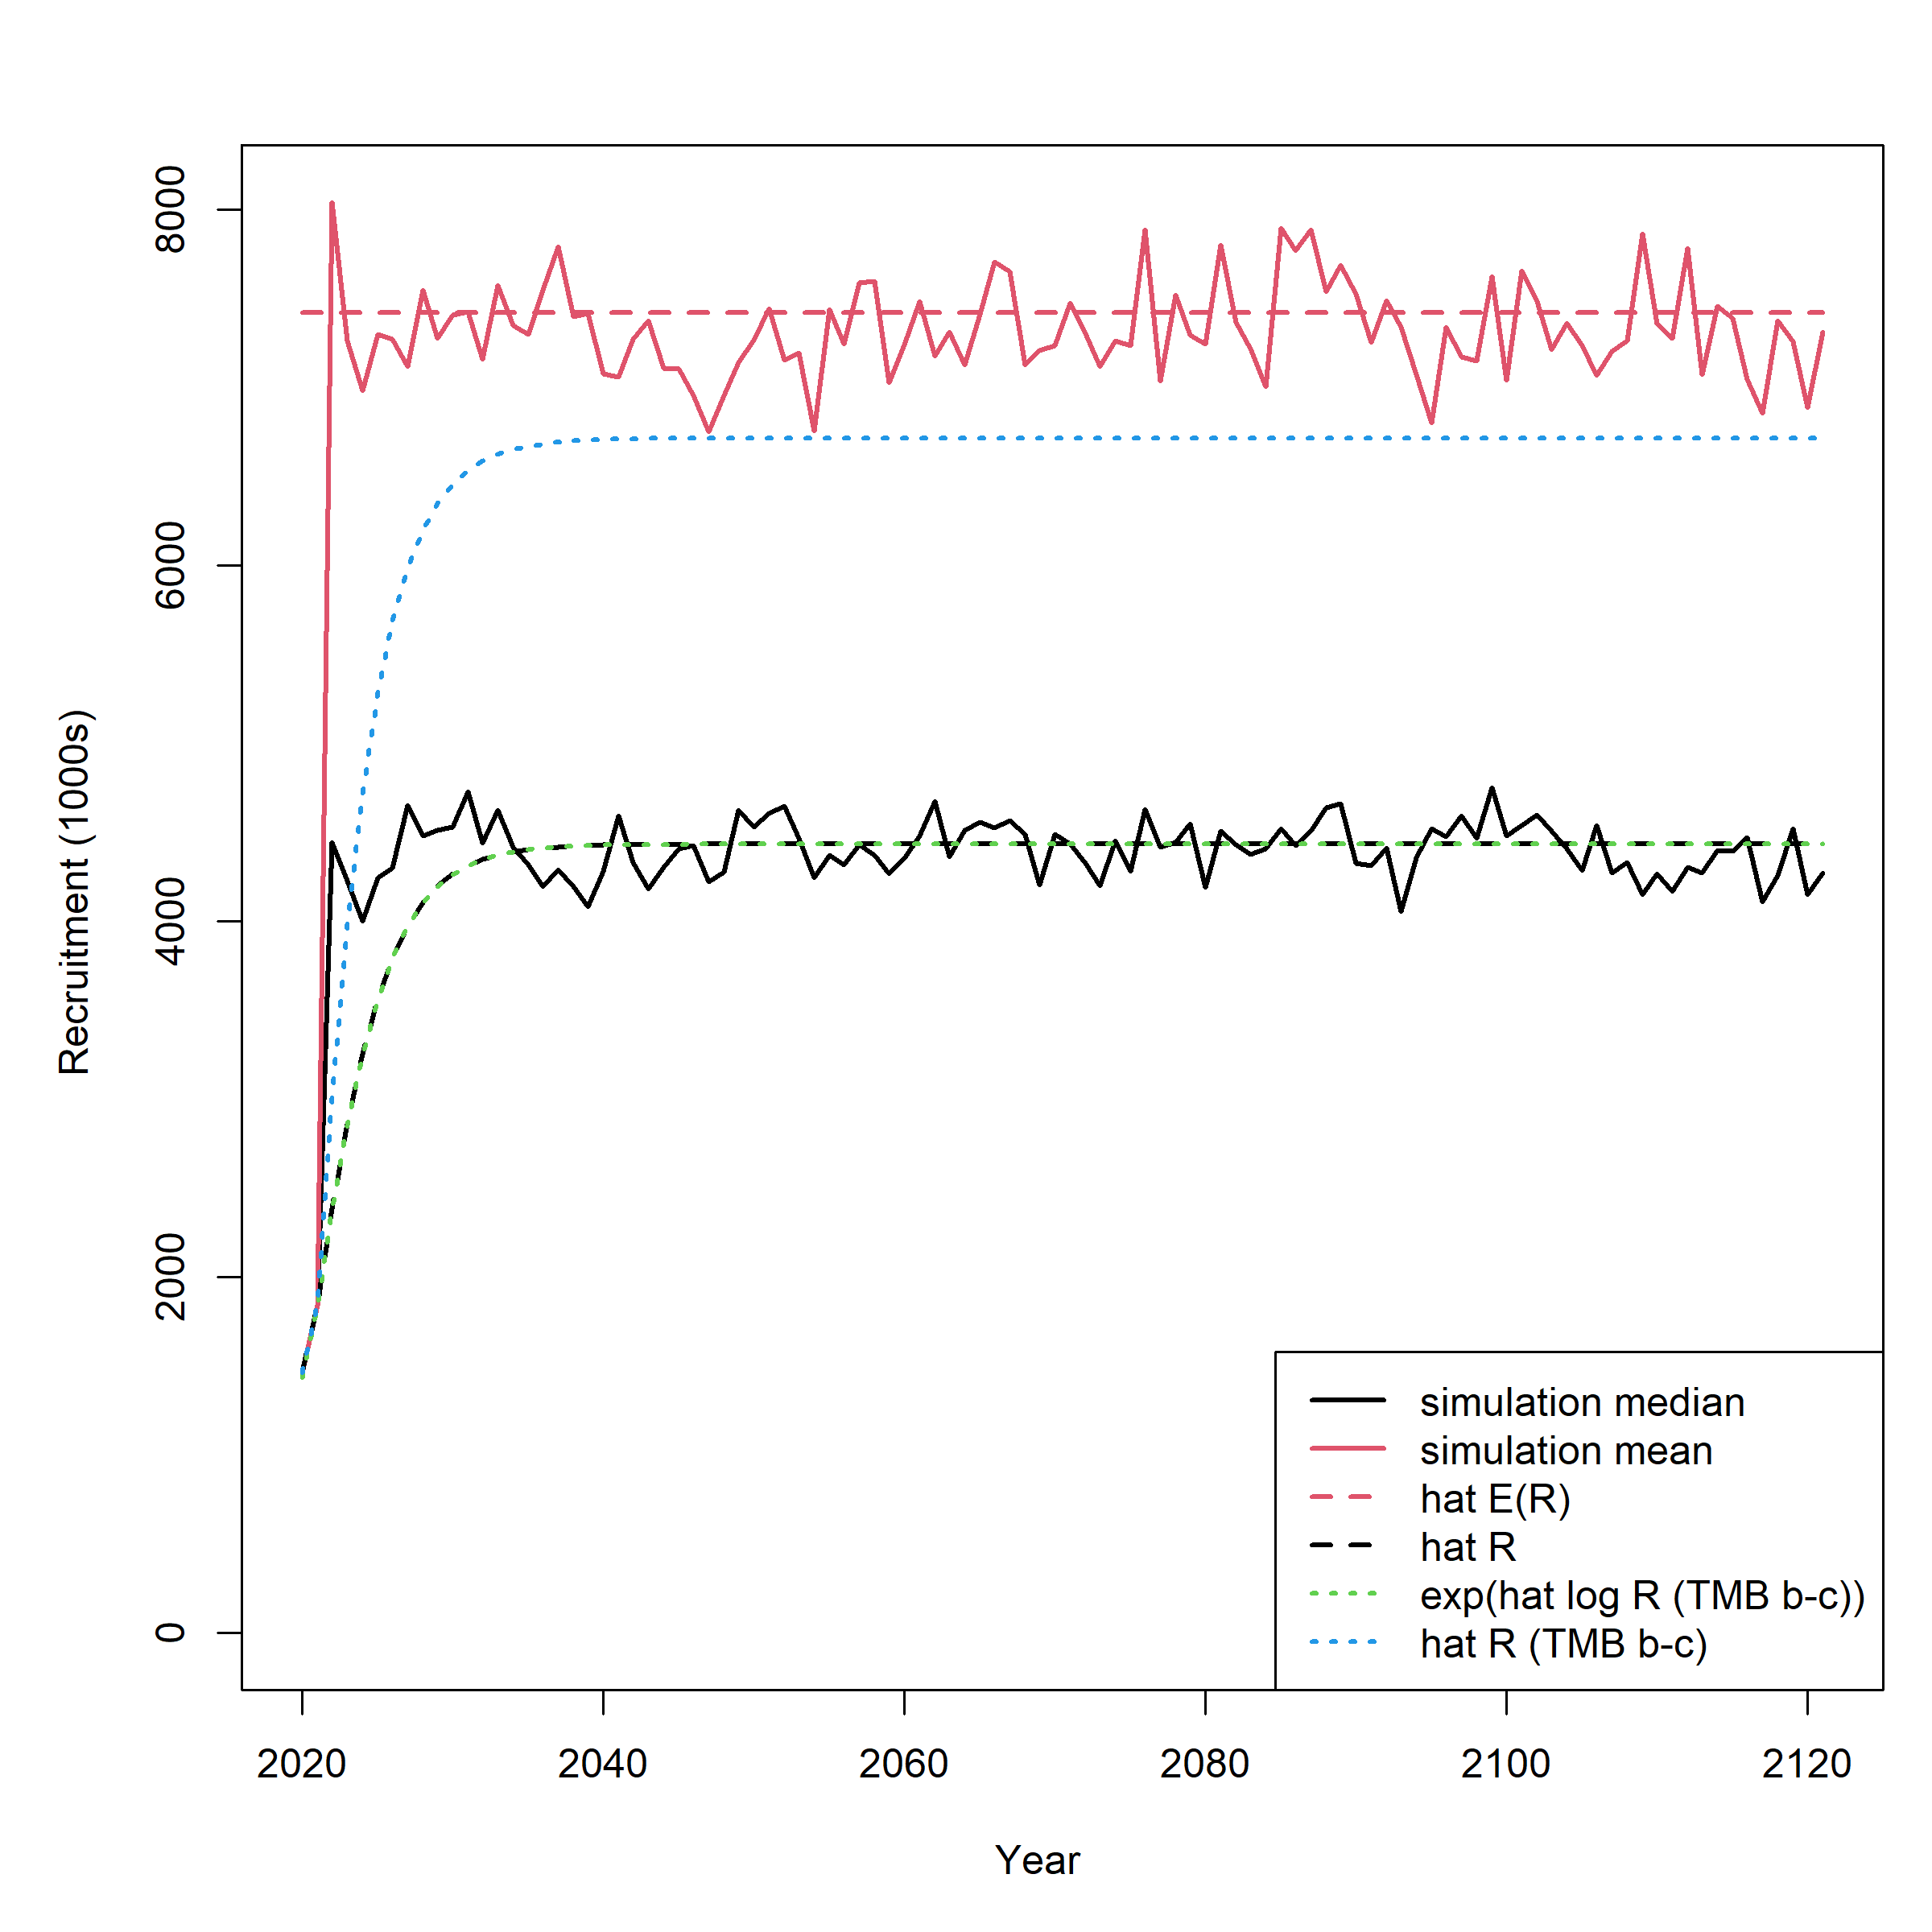
\includegraphics[width=1\linewidth]{compare_recruitment} 

}

\caption{Alternative estimators for projected recruitment in the western Gulf of Maine Atlantic cod WHAM model. Simulation mean and median are that of annual recruitments across simulations. Also shown are the log-normal bias-corrected mean recruitment (hat E(R)), exponential of estimated log-recruit random effects (hat R), and both the exponential of the log-recruit estimate before (hat R (TMB b-c)) and after (exp(hat log R (TMB b-c))) reporting by TMB::sdreport with bias-correction.}\label{fig:recruitment}
\end{figure}

However, neither mean or median spawning biomass can be accurately estimated using analytic methods or model output. When fishing mortality is set at \(F_{40\%}\), the bias-corrected estimator provided by TMB::sdreport is similar to median SSB, but it is supposed to provide an estimate of mean SSB which is unstable but far greater (Fig. \ref{fig:ssb}). The projections at \(F = 0\) suggest the proximity of the bias-corrected estimator to SSB at \(F=F_{40\%}\) is coincidence.

\begin{figure}

{\centering 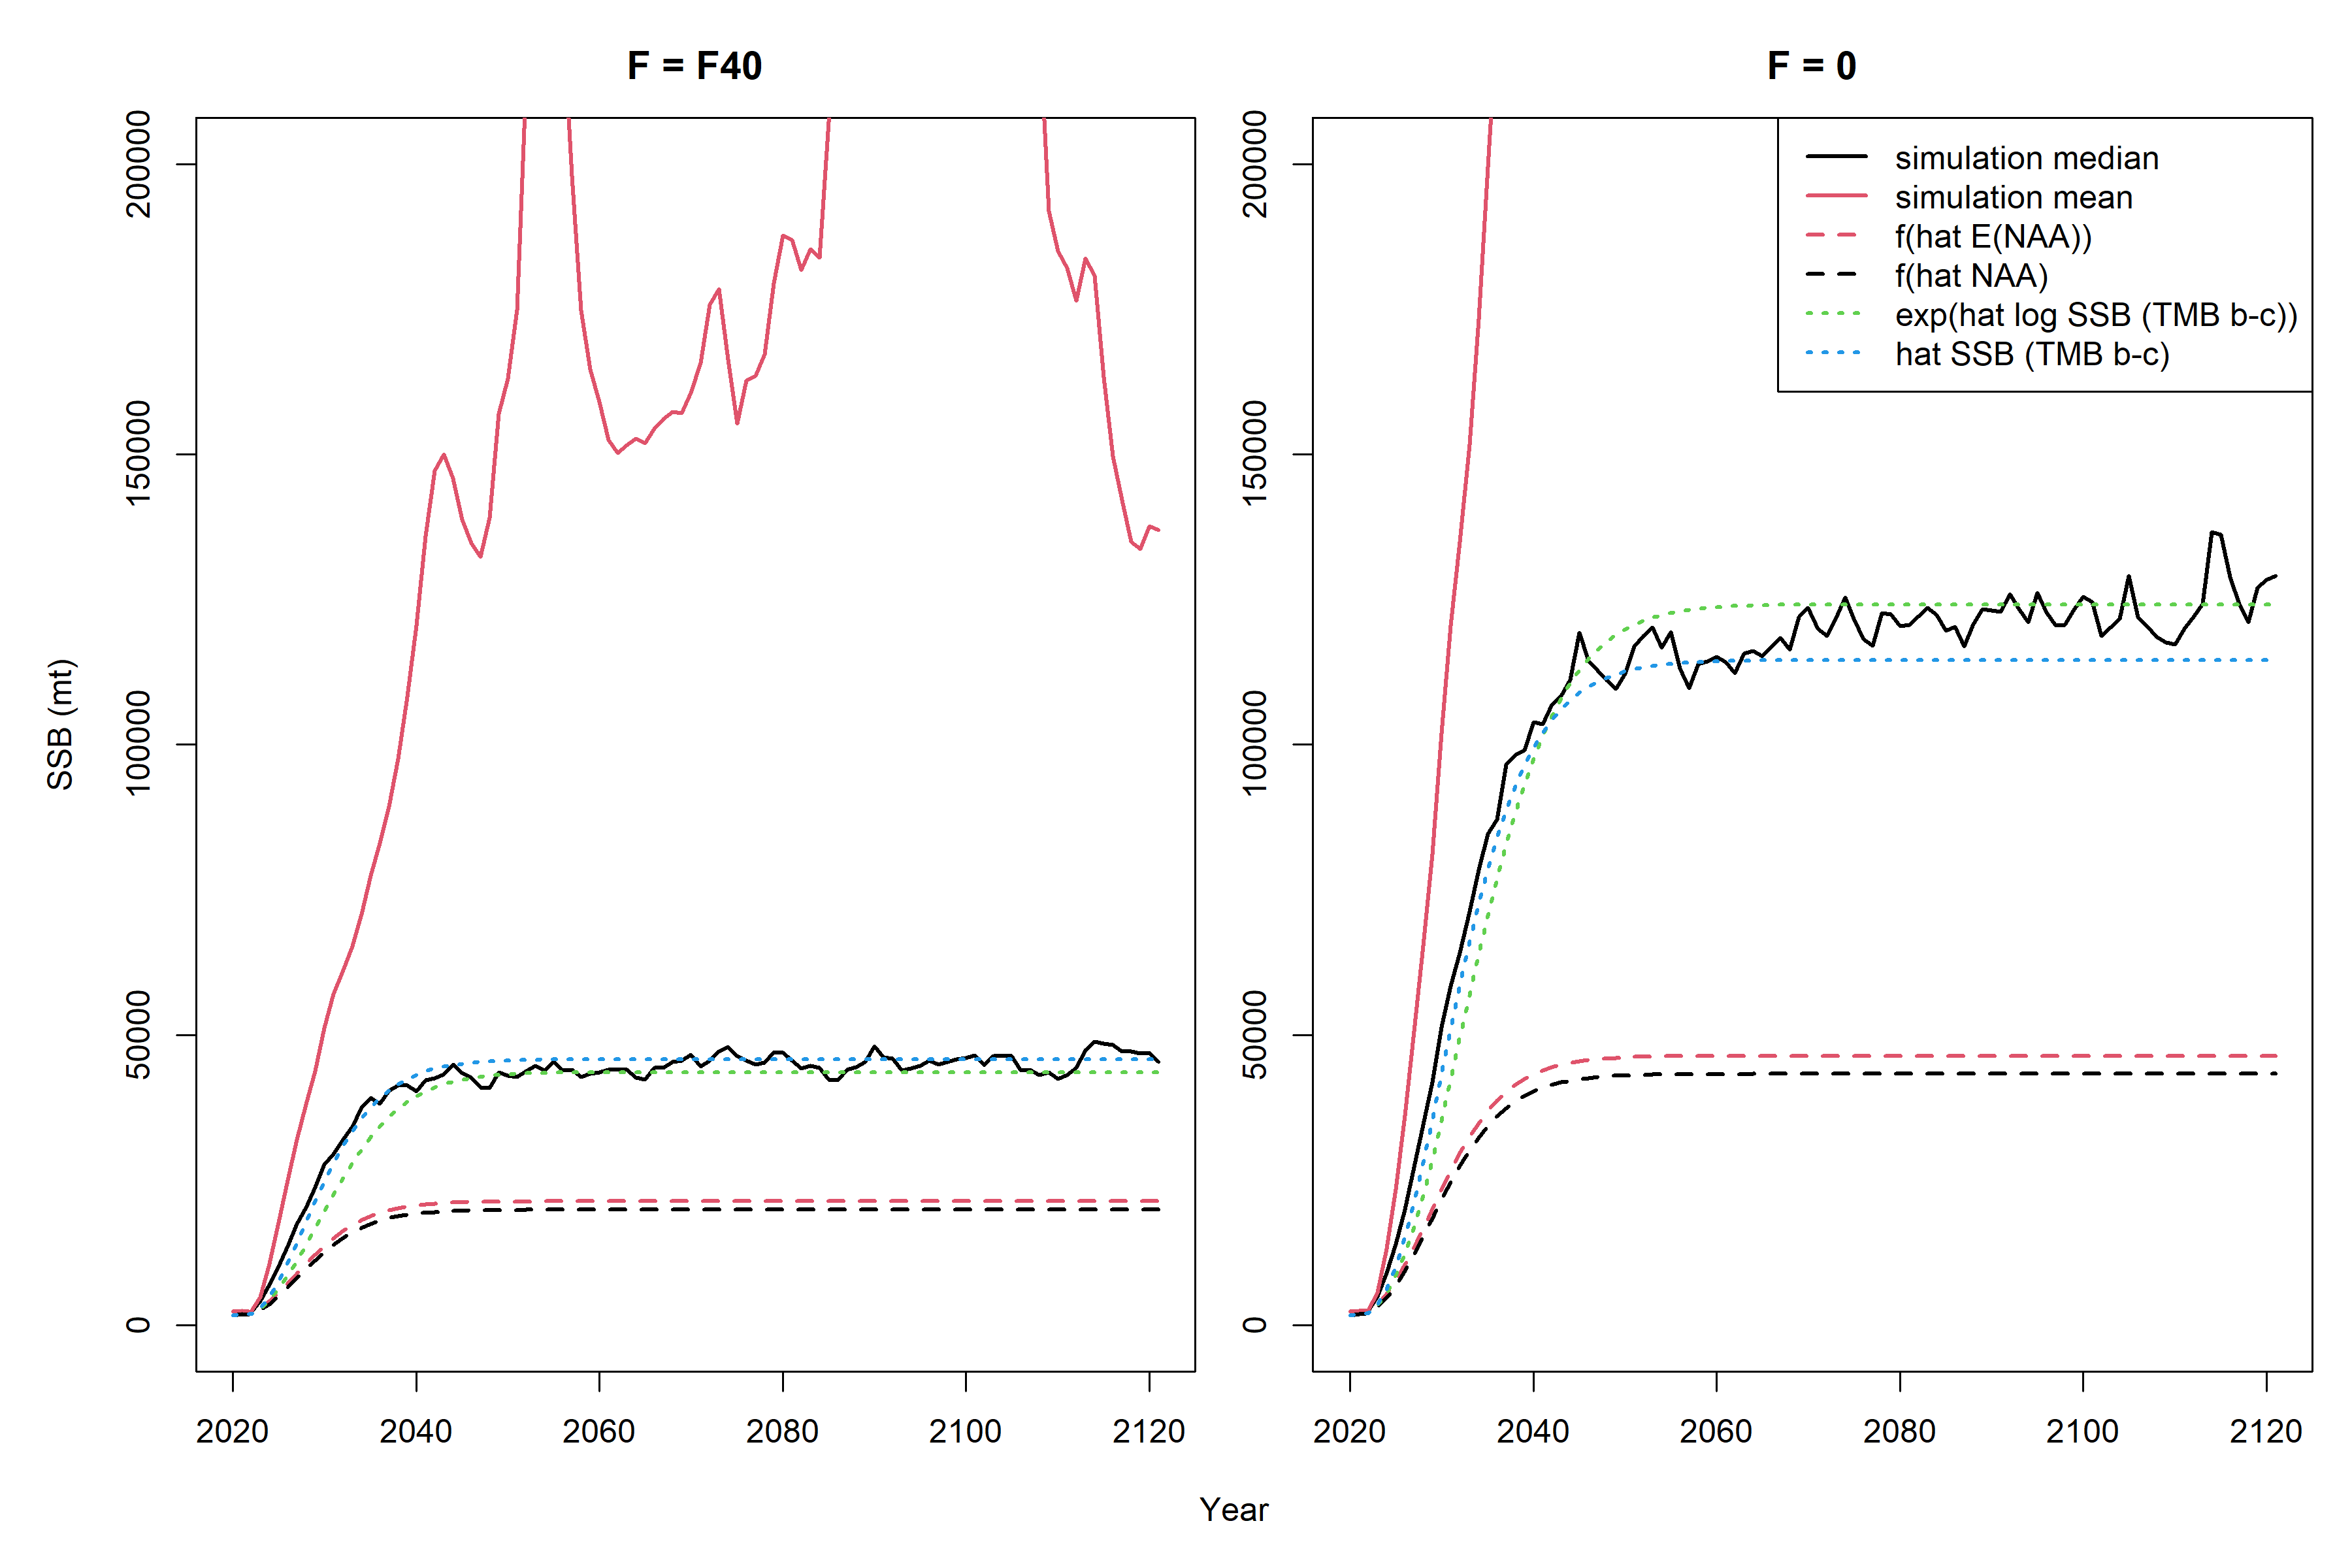
\includegraphics[width=1\linewidth]{compare_ssb} 

}

\caption{Alternative estimators for projected spawning stock biomass (SSB) at $F=F_{40\%}$ (left) or $F=0$ (right) in the western Gulf of Maine Atlantic cod model. Simulation mean and median are that of annual SSB across simulations. Also shown are the SSB calculated from log-normal bias-corrected mean numbers at age (f(hat E(NAA))), from exponential of estimated log-numbers at age random effects (f(hat NAA)), and from either the exponential of the log-SSB estimate before (hat SSB (TMB b-c)) and after (exp(hat log SSB (TMB b-c))) reporting by TMB::sdreport with bias-correction.}\label{fig:ssb}
\end{figure}

By looking at age-specific components of projected SSB we can confirm that median SSB-at-age can only be estimated accurately for the ages prior to the plus group because the plus group is the only age class that is a sum of log-normal random variables (Fig. \ref{fig:ssbaa}). Similarly, the cumulative sum of SSB at age can not be accurately estimated beyond age 1 because it is also the sum of log-normal random variables (Fig. \ref{fig:cumssbaa}).

\begin{landscape}
\begin{figure}

{\centering 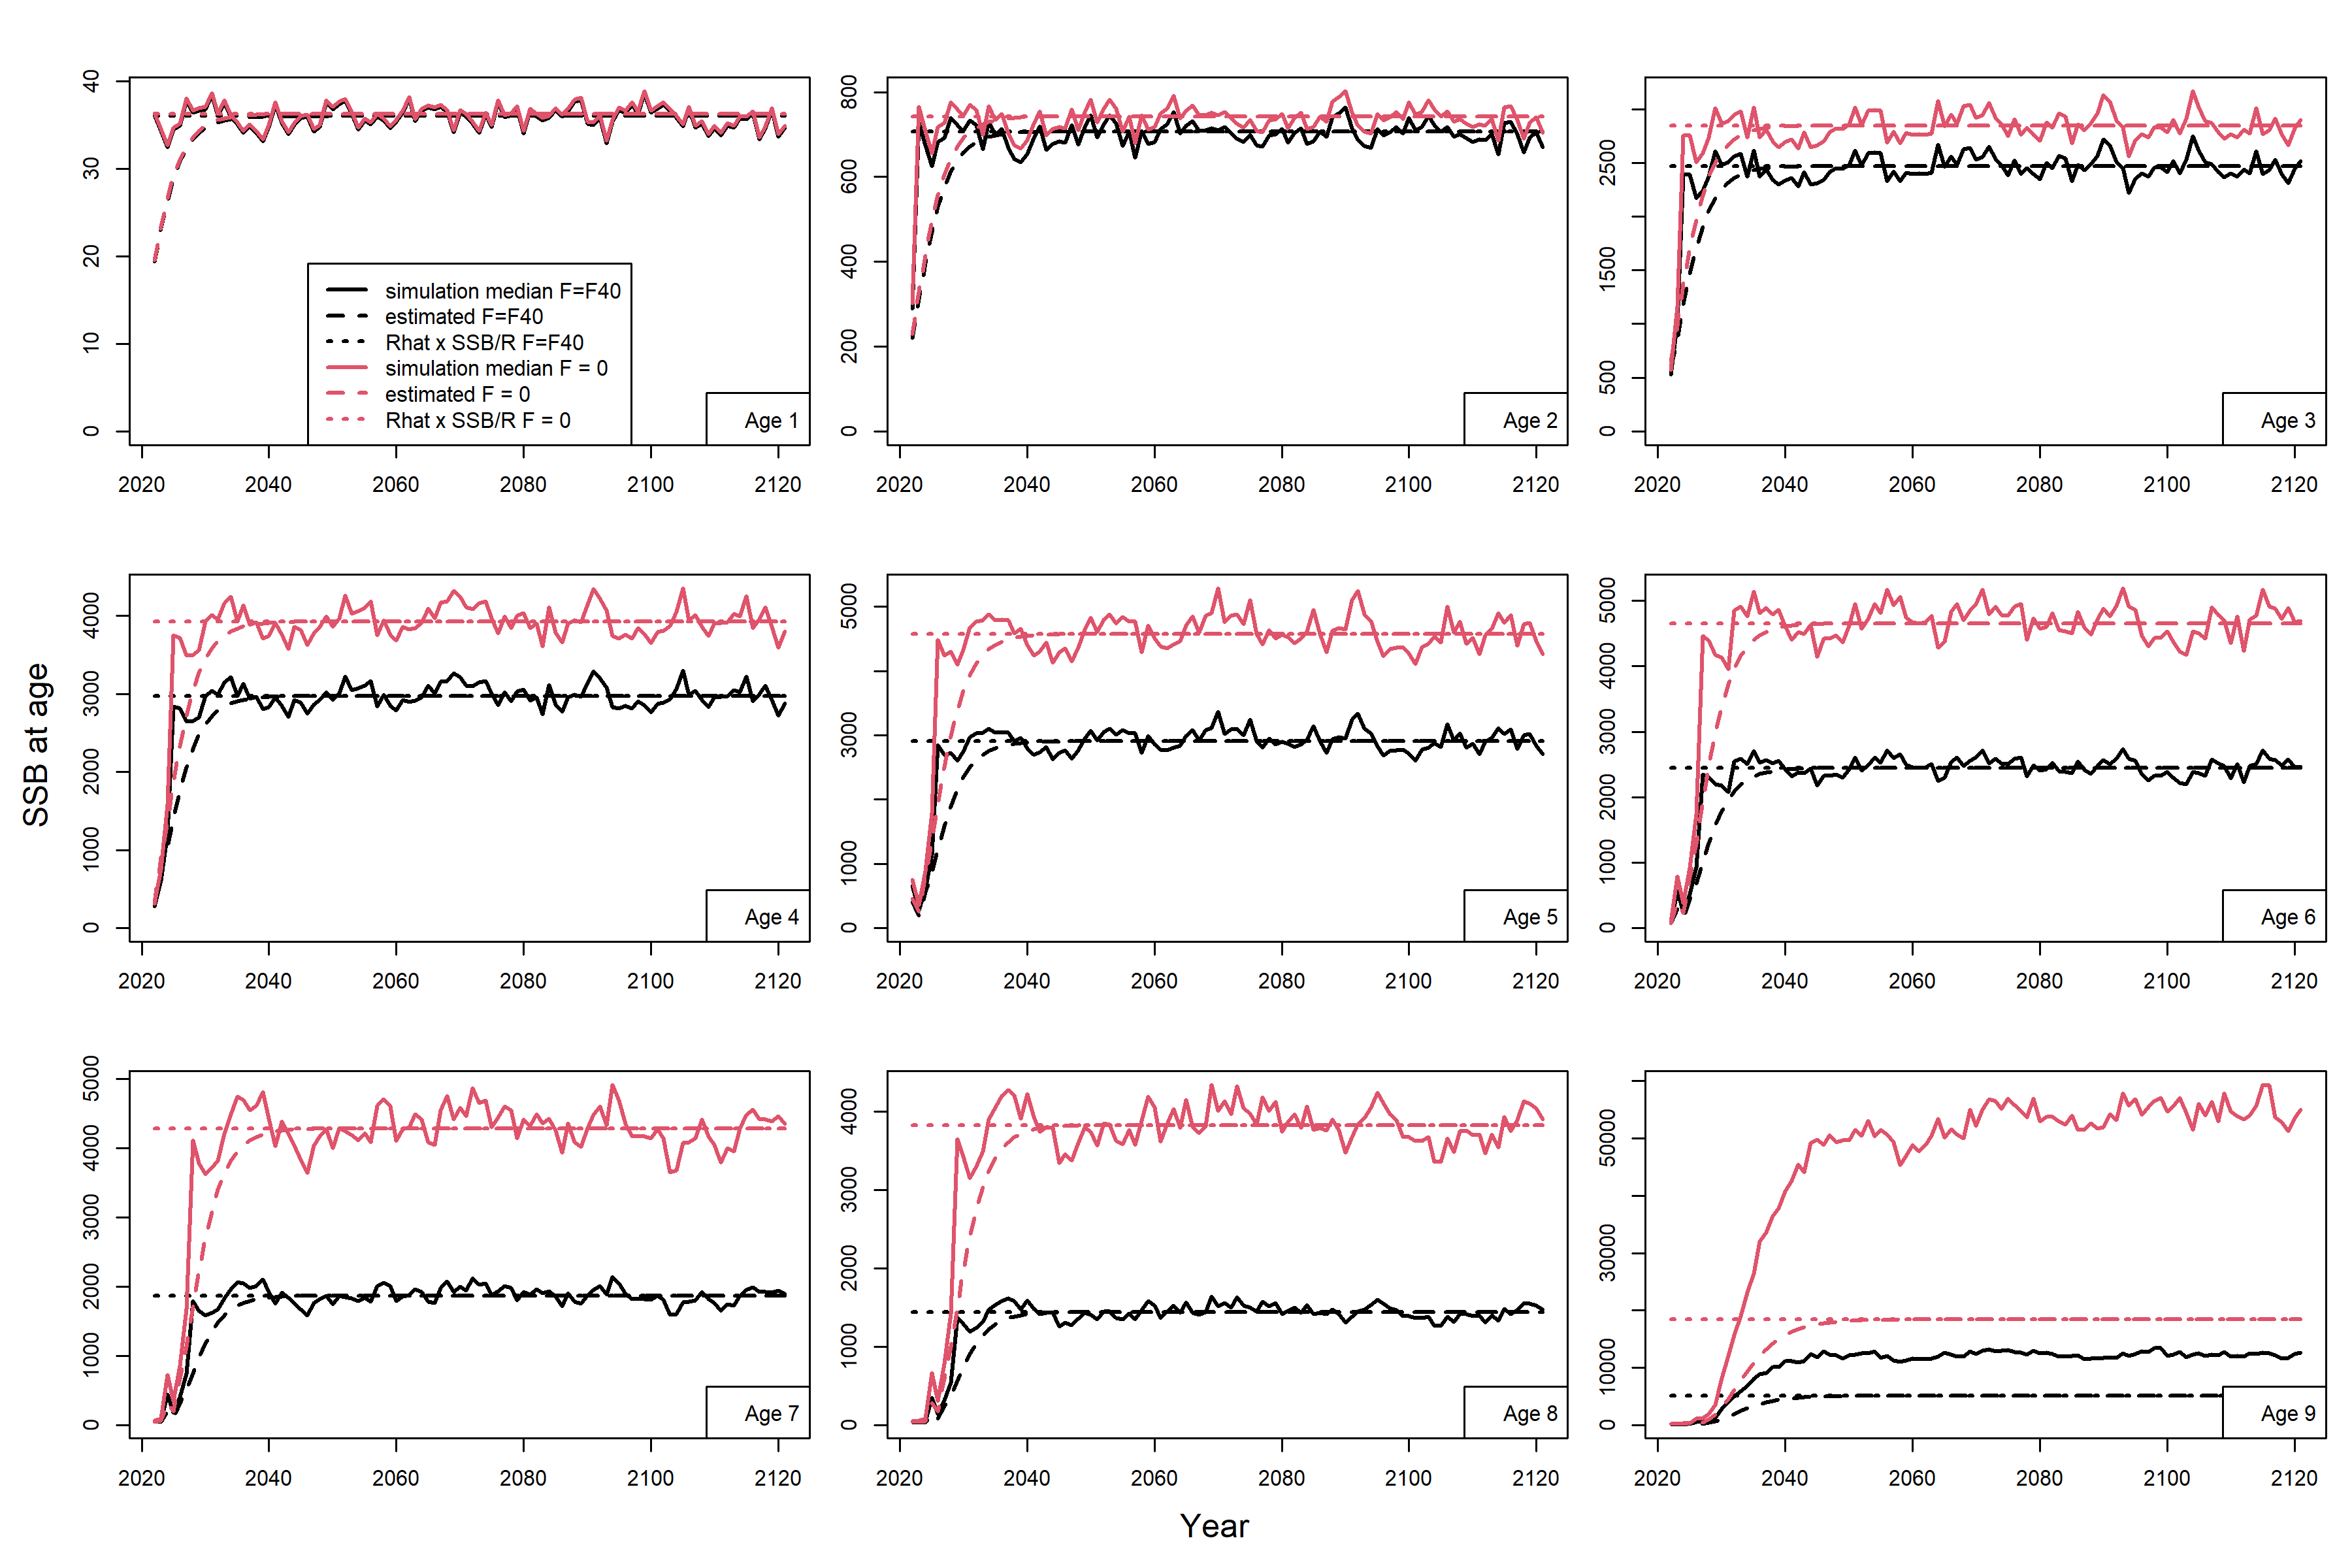
\includegraphics[width=1\linewidth]{compare_SSBAA_F40_at_age} 

}

\caption{Median annual spawning stock biomass at age projected at $F = F40\%$ or $F=0$ across simulations from the western Gulf of Maine Atlantic cod model. Also shown are the SSB as a function of estimated abundance at age (estimated) and the equilibrium SSB calculated as the product of the estimated recruitment and equilibrium SSB/R with log-normal bias-correction (Rhat x SSB/R).}\label{fig:ssbaa}
\end{figure}
\end{landscape}

\begin{landscape}
\begin{figure}

{\centering 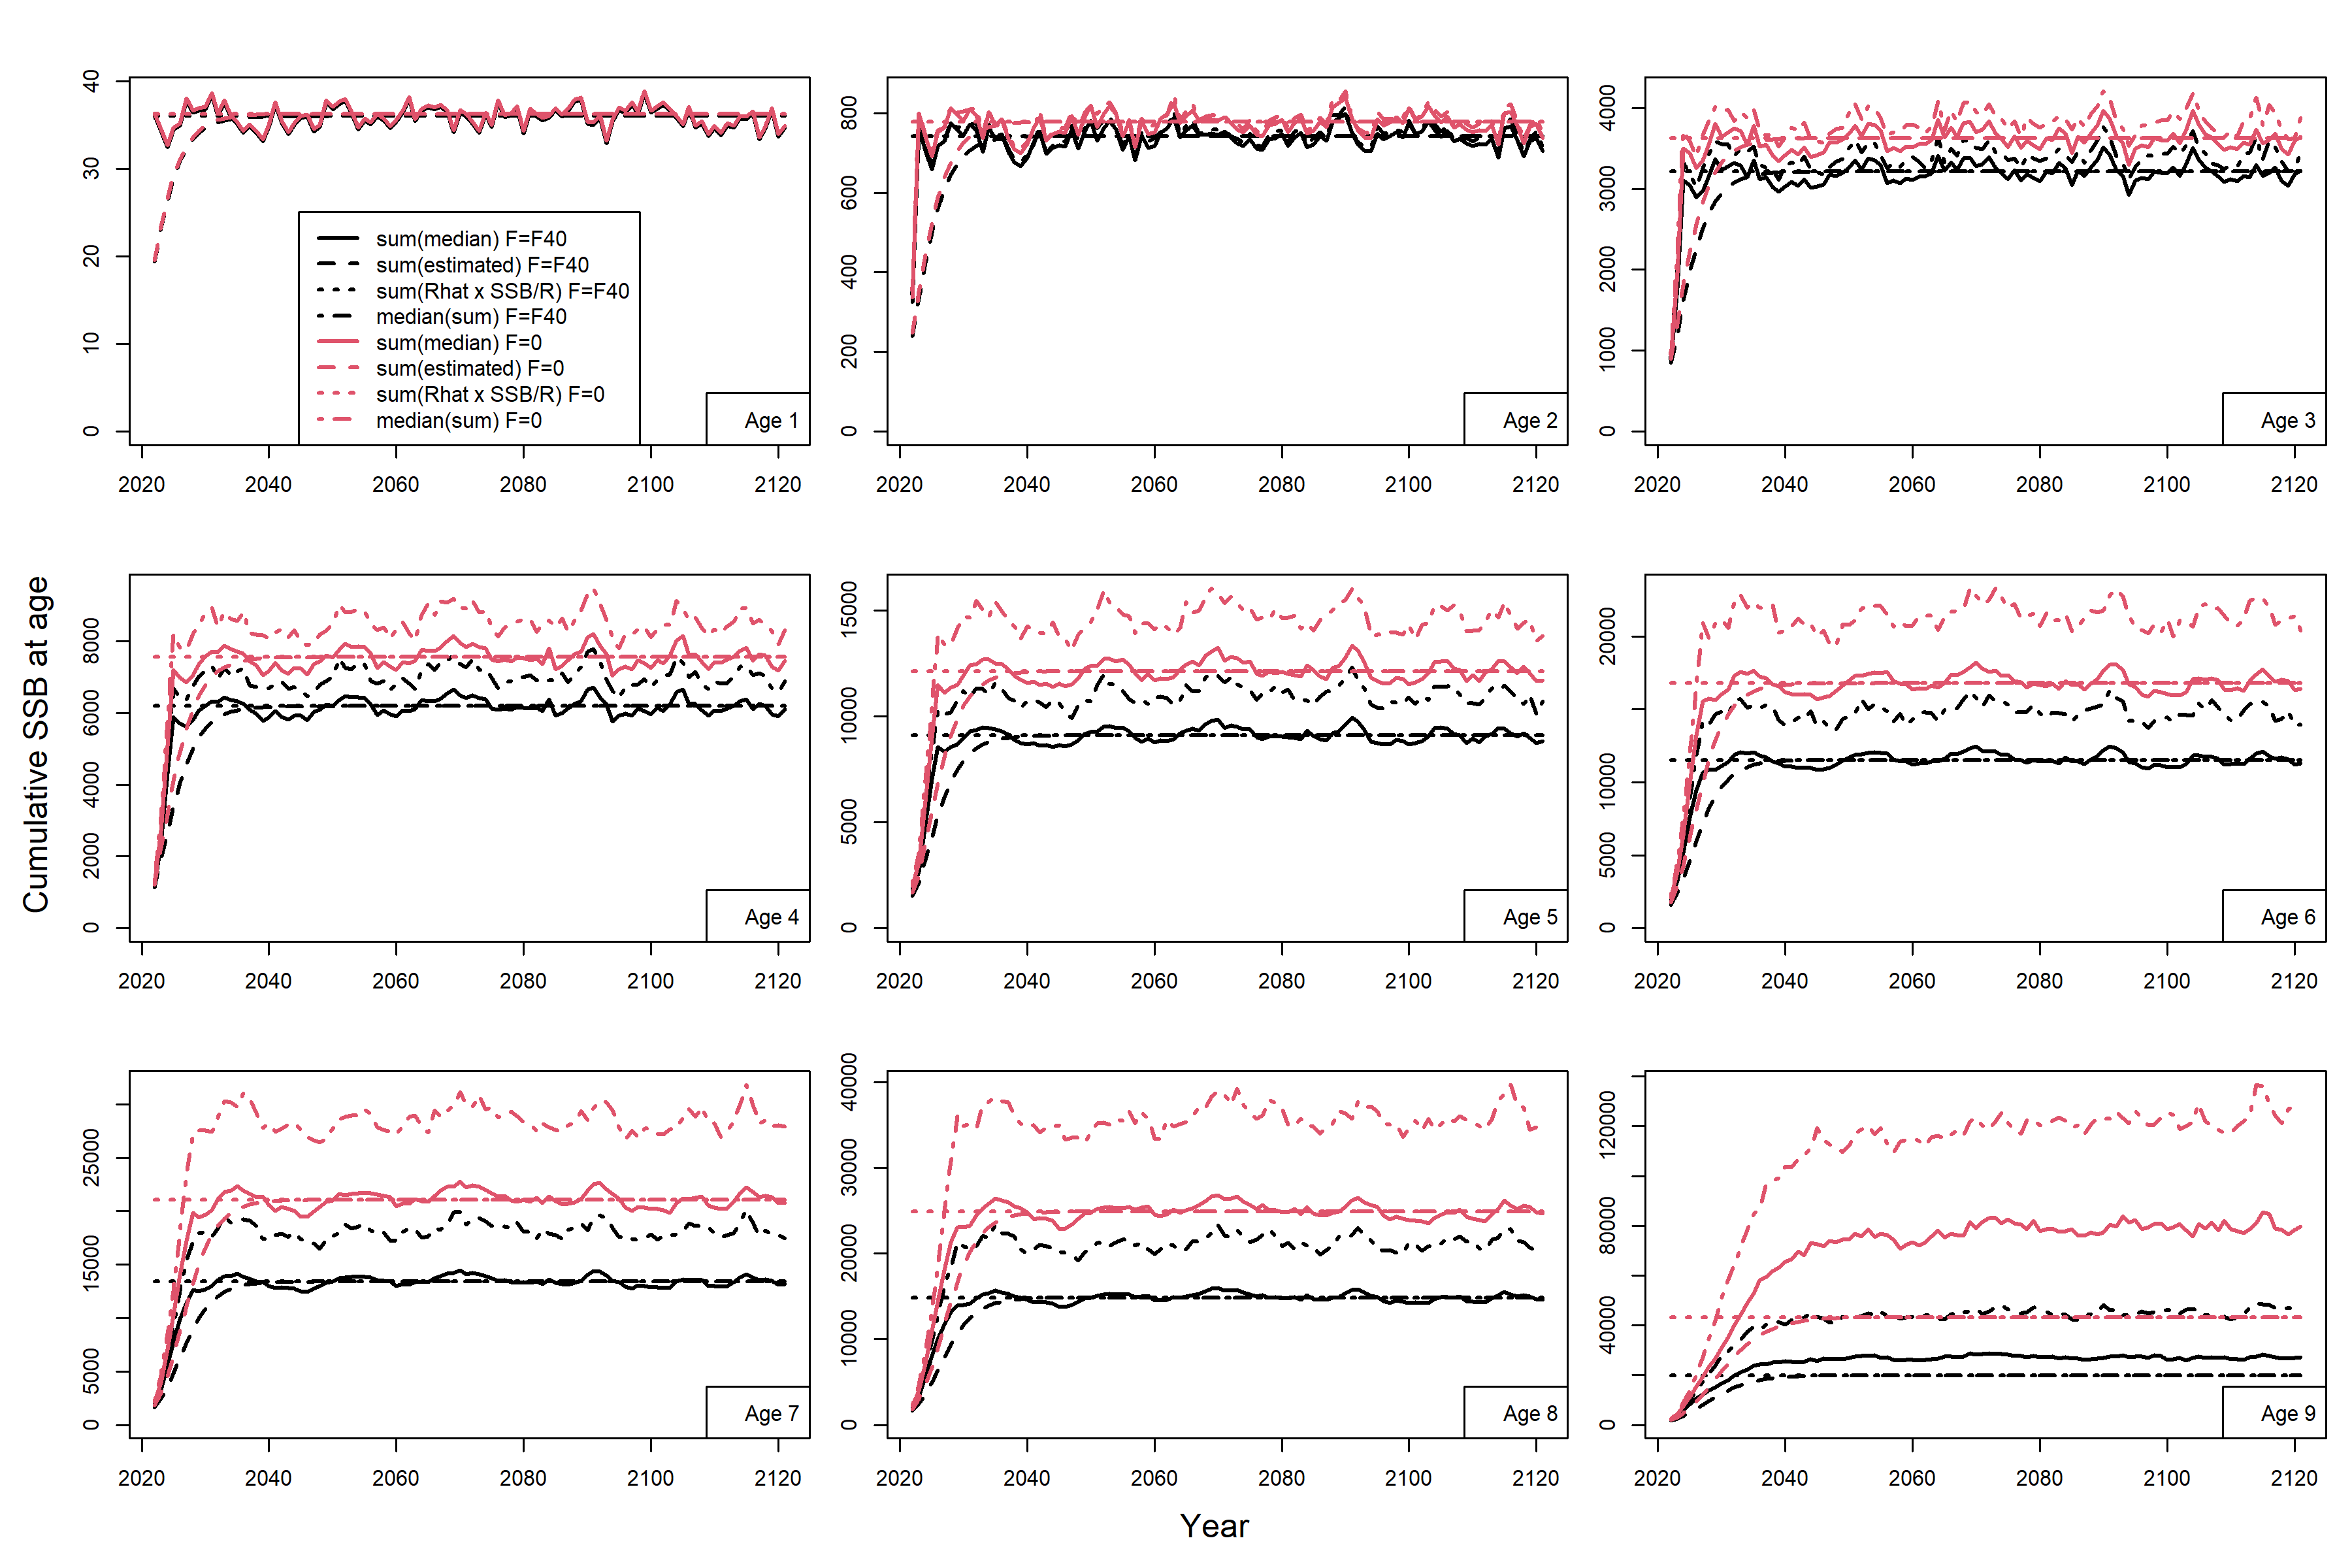
\includegraphics[width=1\linewidth]{compare_cumulative_SSBAA_F40_at_age} 

}

\caption{Median cumulative (median(sum)) or cumulative median (sum(median) spawning biomass at age projected at $F = F40\%$ or $F=0$ across simulations from the western Gulf of Maine Atlantic cod model. Also shown are the cumulative SSB as a function of estimated abundance at age (sum(estimated)) and the cumulative equilibrium SSB calculated as the product of the estimated recruitment and cumulative equilibrium SSB/R at age with log-normal bias-correction (sum(Rhat x SSB/R)).}\label{fig:cumssbaa}
\end{figure}
\end{landscape}

\hypertarget{conclusions}{%
\subsection*{Conclusions}\label{conclusions}}
\addcontentsline{toc}{subsection}{Conclusions}

Analytic estimates of biomass reference points, including are biased for the corresponding median simulated stochastic equilibrium values because the marginal distribution of the simulated values are the sums of log-normal random variables. We showed this for the marginal distribution of equilibrium SSB, and equilibrium SSB in the plus group. However, the median of the equilibrium SSB at each age less than the plus group can be accurately estimated. The demonstration presented assumes stochasticity on abundance at all ages, but this bias would also exist for models with stochasticity only in recruitment (e.g., traditional statistical catch at age models). However, bias in estimation of equilibrium SSB at all ages is expected when a stock-recruit function is used because all ages are then functions of SSB which is the sum of log-normal random variables. Corresponding results are also expected for catch reference points because they are analogous functions of log-normal random variables.

Stochastic equilibrium SSB and catch appears to only be accurately estimated through simulation however determining the appropriate F to obtain the desired percentage of unfished SSB would require simulations to be completed at each F value external to the assessment model rather than internally. Therefore, the uncertainty in parameter estimates from the unprojected model would not be propagated.

If accurate estimation of each of the age-specific components of the biomass or catch reference point is a sufficient goal, then an appropriate expansion of the age classes of the population should minimize any bias in SSB for the plus group.

\end{document}
